\documentclass{article}
\usepackage[english]{babel}
\usepackage{amsmath,amssymb,graphicx,enumerate,hyperref}
\usepackage{geometry} % For page margins 
% \FloatBarrier (as in the placeins package): flush pending figures before each
% (sub)section, so that figures stay inside the subsection that discusses them
\makeatletter
\providecommand\FloatBarrier{\par\begingroup\let\@elt\relax
  \edef\@tempa{\@botlist\@deferlist\@dbldeferlist}%
  \ifx\@tempa\@empty\else\clearpage\fi\endgroup}
\makeatother
%\geometry{a4paper, top=0.6in, bottom=0.8in, left=0.7in, right=0.7in} 
\geometry{a4paper, margin=1in}% Set paper size and margins
\graphicspath{{../figures/}}% figures live in the repository-level figures/ folder

%%%%%%%%%% Start TeXmacs macros
\newcommand{\assign}{:=}
\newcommand{\textdots}{...}
\newcommand{\tmmathbf}[1]{\ensuremath{\boldsymbol{#1}}}
\newcommand{\tmop}[1]{\ensuremath{\operatorname{#1}}}
\newenvironment{enumeratenumeric}{\begin{enumerate}[1.] }{\end{enumerate}}
%%%%%%%%%% End TeXmacs macros



\begin{document}

\title{Convergence study of first order homogenization methods for
steady-state heat conduction in periodically insulated media}

\author{ Hausel-Vargha Emil}

\maketitle

\begin{abstract}
We implement and validate a first-order periodic homogenization method for
steady-state heat conduction in a plate perforated by a periodic array of
insulating holes. The microstructure enters only through a pair of corrector
problems on a single unit cell, which yield an effective conductivity tensor
$\kappa^{\star}$; the macroscopic temperature $T$ is then computed on a hole-free
mesh and the fine-scale field is reconstructed pointwise from the two-scale
expansion $T+\varepsilon\chi\cdot\nabla T$. The method is benchmarked against a
direct numerical solve (DNS) on an exactly matching periodic tiling. With
quadratic finite elements on curved meshes, and meshes refined until the
results no longer change, the finite element error is driven well below the
homogenization error. For a rotated elliptical hole, the RMS error of the
macroscopic field alone decays as $O(\varepsilon^{0.97})$ in the cell size
$\varepsilon$, while the error of the two-scale reconstruction decays as
$O(\varepsilon^{2.02})$: adding the corrector raises the order of accuracy from one
to two, as the asymptotic expansion predicts. The conductivity tensor measured
on a finite perforated sample converges to $\kappa^{\star}$ at rate
$O(\varepsilon)$, with no plateau, for both a circular and an elliptical hole. We
also study how hole shape controls $\kappa^{\star}$: at constant porosity,
elongating an ellipse raises conductivity along its major axis and lowers it
across, while rotating it produces an off-diagonal entry that is largest near
$45^{\circ}$.
\end{abstract}

\clearpage
\tableofcontents
\clearpage

\section{Introduction}

The objective of this study is to verify the convergence of first order
homogenization methods for heat conduction problems in periodically insulated
media. Before homogenization is itself presented, motivation for its use is
given. In particular, the naive approach of a Direct Numerical Solve (DNS) is
discussed as the obvious method for computing the heat field on a perforated
plate. This direct solve uses the Finite Element Method (FEM). Essential to this technique is the variational or weak form of the governing PDE -- here the steady state heat equation -- and as such a derivation of this equation is provided. 
Complementing the derivation is a
brief explanation of how this weak form is used to build the solver for this study. While the DNS is viable and accurate -- so much so that it is used
as a benchmark throughout this investigation -- for a small number of
perforations, it quickly becomes unfeasible once their number increases. This
is primarily because the resolution needed to resolve the effects of many
small inclusions is too expensive and the simulation fails to terminate within
a reasonable time frame. Also, the computational domain to mesh becomes much
more complicated, to the extent that even building the geometry becomes
expensive. To combat these effects, a first order homogenization method is
introduced to solve a simpler problem and reconstruct the solution function
without needing to produce complicated geometries or solve equations on them.
The results of the this new, homogenized simulation are then presented and discussed before some brief concluding remarks are made to close the study.

\FloatBarrier
\section{DNS - Heat conduction and the Finite Element Method}

This section provides the ingredients needed for the naive DNS. The heat
equation, boundary conditions, weak form, and FEM are discussed.

\FloatBarrier
\subsection{The heat equation - governing physics}

Consider a bounded domain $\Omega \subset \mathbb{R}^2 $, with boundary
$\partial \Omega$. The temperature $u (\tmmathbf{x}, t)$ obeys the general
time-dependent heat equation
\begin{equation}
  \label{eq:heat_general}
  \left\{ \begin{array}{c}
    \nabla \cdot (\kappa \nabla u) + Q = \rho c_p \frac{\partial u}{\partial
    t}, \quad \tmop{on} \Omega\\
    \tmop{boundary} \tmop{condition}, \quad \tmop{on} \partial \Omega \\
    u\equiv u_0, \quad t=0
  \end{array} \right.
\end{equation}
where
\begin{itemize}
  \item $\kappa (\tmmathbf{x})$ is the conductivity tensor
  
  \item $\rho$ is the mass density of the medium
  
  \item $c_p$ is the heat capacity at constant pressure
  
  \item $Q$ is the total of all heat sources
\end{itemize}
In our study, the equation is drastically simplified so that emphasis may be
placed on the numerical homogenization methods as opposed to sophisticated physics.
In particular, the following assumptions are made:
\begin{enumeratenumeric}
  \item There are no sources or sinks in the plate (i.e. $Q = 0$)
  
  \item The plate has reached a steady-state temperature and (no time dependence,
  $\partial_t u = 0$)
  
  \item Conductivity $\kappa$ is constant and isotropic throughout the solid
  material (i.e. $\kappa$ is a scalar everywhere it is defined)
\end{enumeratenumeric}
Thus the problem transforms from an initial-boundary value problem to a boundary value problem. One might, of course, extend the analysis to the time-dependent case, whereby
the physical quantities of interest could become the speed of heat
propagation, transient storage, time constants, and thermal lag. This is an
interesting problem in its own right, however the implementation is even more
involved. With the assumptions above, Eq.~\eqref{eq:heat_general} reduces to
\begin{equation}
  \label{eq:heat_steady}
  \left\{ \begin{array}{c}
    \nabla \cdot (\kappa \nabla u) = 0, \quad \tmop{on} \Omega\\
    \tmop{boundary} \tmop{condition}, \quad \tmop{on} \partial \Omega
  \end{array} \right.
\end{equation}
with $u = u (x)$ and $x = (x_1, x_2) \in \Omega$. This is the final, simplified equation which is used to
govern the physics throughout the study.

\FloatBarrier
\subsection{Equation domain and boundary conditions}
\label{sec:domain}

In order for the problem to be well posed, one must put into place the
boundary conditions. The case of interest is when the domain has periodic
inclusions made of an entirely insulating medium, that is, there are
periodic occurrences of regions where $\kappa = 0$. In order to recreate this
numerically a rectangular domain is used, which is then perforated with
regularly spaced circular holes. Perfect insulation is simulated by imposing a
Neumann boundary condition: through the surface of each such inclusion zero
heat flux is allowed. Further, the quantity of interest in this study is the
effective conductivity tensor $\kappa^{\star}$ of the resulting material. To
gain information about this tensor, a macroscopic temperature gradient is
imposed laterally on the whole domain. This is done by choosing Dirichlet boundary
conditions. Finally, in order to avoid heat leakage through the bottom and top edges of the rectangle, zero heat flux is required through these edges also. A summary of these conditions, on the domain $\Omega = [0, L_1] \times [0, L_2]$, is given below
\begin{equation}
  \label{eq:bc}
  \tmop{BC} = \left\{ \begin{array}{l}
    u (0, x_2) = 0 \quad \forall x_2 \in [0, L_2] \\
    u (L_1, x_2) = 1 \quad \forall x_2 \in [0, L_2] \\
    \nabla u \cdot \mathbf{n}= 0 \quad \tmop{on} y_{\min}, \, y_{\max}
    \tmop{edges}\\
    \nabla u \cdot \mathbf{n}= 0 \quad \tmop{on} \tmop{inclusion} \tmop{edges}
  \end{array} \right.
\end{equation}
A sketch of these conditions can be found in Fig.~\ref{fig:bc_dns}(a), and an example mesh, as used in
the computations, is shown in Fig.~\ref{fig:perforated_rectangle}.

\begin{figure}[h]
  \centering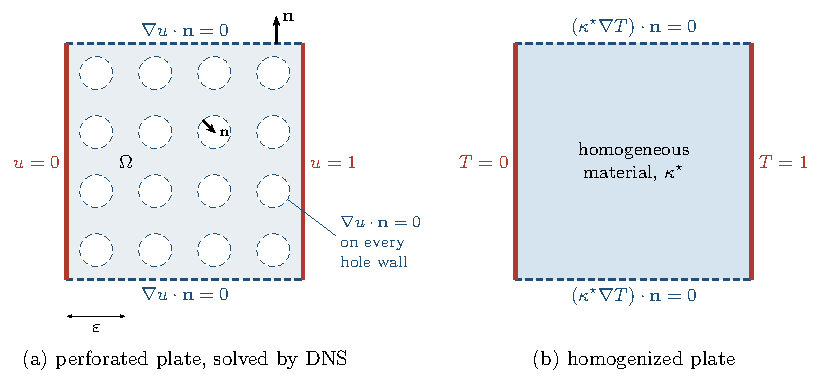
\includegraphics[width=0.95\textwidth]{bc_dns.pdf}
  \caption{Boundary conditions of the two problems posed on the plate. (a) The direct
  numerical solve of Eq.~\eqref{eq:heat_steady} with the conditions of
  Eq.~\eqref{eq:bc}, where the temperature is imposed on the left and right edges
  and no heat crosses the top and bottom edges or the wall of any hole, $\mathbf{n}$
  being the outward normal of $\Omega$, which points into the holes. (b) The
  homogenized problem of Eq.~\eqref{eq:macro_problem}, posed on the same square
  without holes, with the same imposed temperatures and with insulated top and
  bottom edges, where the zero-flux condition now involves the effective tensor
  $\kappa^{\star}$.}
  \label{fig:bc_dns}
\end{figure}

One could extend the study to three dimensions, in which case the domain would
resemble the one shown in Fig.~\ref{fig:perforated_cube} in the appendix. A slice of the direct numerical solve for a simple 10 by 10 case can be seen in Fig.~\ref{fig:cube_temperature}. The cube is sliced to reveal the temperature inside it, which varies across the cylinders but not along them. Perforating a cube with simple parallel cylinders is, by symmetry, exactly equivalent to completing a simpler 2D study of the perpendicular cross-section, which is what is done here; reducing dimensions substantially reduces computational costs. It would be interesting, however, to
study the effect of rotating or curving the inclusions on the effective
conductivity tensor. One might ask if any $\kappa^{\star}$ can be attained by
playing with the geometry.

\FloatBarrier
\subsection{Variational form}

\FloatBarrier
\subsubsection{General presentation}

Finding the variational or weak form of a partial differential equation is the
first step in most finite element techniques. Not every PDE admits one: the
construction below relies on integrating by parts, which requires the equation
to have a suitable structure. Whether a given problem has a weak
form therefore has to be checked, and the next subsection does this for the
heat equation considered here. Given a boundary value problem
$\Xi$ over a domain $\Omega$, let $V$ be the general solution space. Define
further $\partial \Omega_{\tmop{Dirichlet}}$ and $\partial
\Omega_{\tmop{Neumann}}$ as the parts of the boundary where Dirichlet or
Neumann boundary conditions are applied, respectively. The variational form is
obtained, in general, by multiplying both sides of the partial differential
equation with a test function
\[ v \in V^0 \assign \left\{ f \in V : f (\mathbf{x}) = 0 \quad \forall
   \mathbf{x} \in \partial \Omega_{\tmop{Dirichlet}}  \right\} \]
Then through integration by parts and integral identities, one obtains an
equation of the form
\begin{equation}
  \label{eq:weak_general}
  a (u, v) = L (v) \quad \forall v \in V^0
\end{equation}
for some linear form $L : V \rightarrow \mathbb{R}$ and bilinear form $a : V
\times V \rightarrow \, \mathbb{R}$, which must be satisfied by $u$. Once the problem is rewritten in this
way, the infinite dimensional solution space $V$ is approximated by a finite
dimensional space $V_h$ with a well chosen basis $\{ v^i_h \}_{i = 1}^n$ of
functions. These functions are called ``finite elements''. In effect, the
essence of the method consists in approximating the unknown function by
assuming it is made up of a linear combination of these finite elements, and
then determining the weight of each using Eq.~\eqref{eq:weak_general}. In a
finite dimensional space, a bilinear form can be represented by its associated
matrix $\mathbf{A}$, and a linear form by a vector of its coefficients in the
dual space $\tmmathbf{l}$. In this way, Eq.~\eqref{eq:weak_general} reduces to
a linear problem
\[ \mathbf{v}^\mathsf{T}\mathbf{A}\mathbf{u}=\mathbf{v}^\mathsf{T}\tmmathbf{l}\quad \forall\mathbf{v}\in V^0_h \iff \mathbf{A}\mathbf{u}=\tmmathbf{l} \]
Further, the finite elements are generally chosen to be equal to 1 at their
node on the mesh, and to decrease to zero everywhere else. As a result, the
weights in front of each element are in fact equal to the value of the unknown
function $u$ at the corresponding node. A typical example would be the hat
functions, or 1st order Lagrange elements. See
https://jsdokken.com/FEniCS-workshop/README.html for a more comprehensive
presentation of the finite elements.



\FloatBarrier
\subsubsection{Application }
\label{sec:application}

Consider again the boundary value problem in Eq.~\eqref{eq:heat_steady}, with the
boundary conditions of Eq.~\eqref{eq:bc}. Take $V = C^2 (\bar{\Omega})$, the set of
twice differentiable functions on the closure of $\Omega$. We show that this
problem admits a weak form, in three steps:
\begin{enumeratenumeric}
  \item starting from the PDE, we derive an equation of the form
  Eq.~\eqref{eq:weak_general};
  \item we state the resulting weak form, for the boundary conditions used here
  and for more general Neumann data;
  \item we show the converse: a function satisfying the weak form (and the
  Dirichlet conditions) solves the PDE and satisfies the Neumann conditions.
\end{enumeratenumeric}
Steps 1 and 3 together show that solving the weak form is equivalent to solving
the original problem, which is what justifies using it in the solver.

Throughout, $\mathbf{n}$ is the outward unit normal on $\partial\Omega$, $dl$ the
length element along the boundary, and $d\mathbf{l} = \mathbf{n}\, dl$ the
corresponding normal vector element.

\paragraph{Step 1: from the PDE to the weak form.} Let $u$ solve
Eq.~\eqref{eq:heat_steady}, and multiply by any $v \in V^0$. Since $\kappa$ is a
non-zero constant,
\begin{eqnarray*}
  & \nabla \cdot (\kappa \nabla u) = 0 &  \\
  \Rightarrow & \Delta u \, v = 0 &  \\
  \Rightarrow & \displaystyle\iint_{\Omega} \Delta u \, v \, d\Omega = 0 &  \\
  \Rightarrow & \displaystyle\iint_{\Omega} \nabla \cdot (v \nabla u) \, d\Omega - \iint_{\Omega}
  \nabla u \cdot \nabla v \, d\Omega = 0 &  \\
  \Rightarrow & \displaystyle\oint_{\partial \Omega} v \nabla u \cdot d\mathbf{l} -
  \iint_{\Omega} \nabla u \cdot \nabla v \, d\Omega = 0 & \forall v \in V^0
\end{eqnarray*}
where the fourth line uses the product rule $\nabla \cdot (v \nabla u) = \nabla u
\cdot \nabla v + v \Delta u$ and the last one the divergence theorem. Splitting
the boundary integral,
\[ \oint_{\partial \Omega} v \nabla u \cdot d\mathbf{l} = \int_{\partial
   \Omega_{\tmop{Dirichlet}}} v \nabla u \cdot d\mathbf{l} \, + \, \int_{\partial
   \Omega_{\tmop{Neumann}}} v \nabla u \cdot d\mathbf{l} . \]
The first term is null because $v = 0$ on $\partial \Omega_{\tmop{Dirichlet}}$ by definition.
The second is null because the Neumann conditions give $\nabla u \cdot d\mathbf{l}
= (\nabla u \cdot \mathbf{n}) \, dl = 0$ on $\partial \Omega_{\tmop{Neumann}}$.

\paragraph{Step 2: the weak form.} We are left with
\begin{equation}
  \label{eq:weak_final}
  \iint_{\Omega} \nabla u \cdot \nabla v \, d\Omega = 0 \quad \forall v \in V^0
\end{equation}
which is of the form of Eq.~\eqref{eq:weak_general}, with
\[ a (u, v) = \iint_{\Omega} \nabla u \cdot \nabla v \, d\Omega \,, \quad L (v) = 0 . \]
The Dirichlet conditions do not appear in Eq.~\eqref{eq:weak_final}: they are
imposed on $u$ directly, and through the choice $v \in V^0$. The Neumann
conditions, on the other hand, are contained in the linear form $L$. With a
general Neumann condition $\nabla u \cdot \mathbf{n} = g \in C^0 (\partial
\Omega_{\tmop{Neumann}})$, the second boundary term in Step 1 no longer vanishes but
equals $\int_{\partial \Omega_{\tmop{Neumann}}} g v \, dl$, and the same derivation
gives
\begin{equation}
  \label{eq:weak_neumann}
  \iint_{\Omega} \nabla u \cdot \nabla v \, d\Omega = \int_{\partial
  \Omega_{\tmop{Neumann}}} g v \, dl \quad \forall v \in V^0 ,
  \qquad \text{i.e.} \quad L (v) = \int_{\partial \Omega_{\tmop{Neumann}}} g v \, dl .
\end{equation}
Our problem is the case $g = 0$.

\paragraph{Step 3: from the weak form back to the PDE.} Conversely, let $u \in V$
satisfy the Dirichlet conditions and Eq.~\eqref{eq:weak_neumann}. Running the
integrations by parts of Step 1 backwards,
\begin{eqnarray*}
  & \displaystyle\iint_{\Omega} \nabla u \cdot \nabla v \, d\Omega = \int_{\partial
  \Omega_{\tmop{Neumann}}} g v \, dl &  \\
  \Rightarrow & \displaystyle\iint_{\Omega} \nabla \cdot (v \nabla u) \, d\Omega -
  \iint_{\Omega} \Delta u \, v \, d\Omega = \int_{\partial \Omega_{\tmop{Neumann}}} g v
  \, dl &  \\
  \Rightarrow & \displaystyle\oint_{\partial \Omega} v \nabla u \cdot d\mathbf{l} -
  \iint_{\Omega} \Delta u \, v \, d\Omega = \int_{\partial \Omega_{\tmop{Neumann}}} g v
  \, dl &  \\
  \Rightarrow & \displaystyle\iint_{\Omega} \Delta u \, v \, d\Omega = \int_{\partial
  \Omega_{\tmop{Dirichlet}}} v \nabla u \cdot d\mathbf{l} + \int_{\partial
  \Omega_{\tmop{Neumann}}} v \nabla u \cdot d\mathbf{l} - \int_{\partial
  \Omega_{\tmop{Neumann}}} g v \, dl & 
\end{eqnarray*}
and, since $v = 0$ on $\partial \Omega_{\tmop{Dirichlet}}$,
\begin{equation}
  \label{eq:weak_converse}
  \iint_{\Omega} \Delta u \, v \, d\Omega = \int_{\partial \Omega_{\tmop{Neumann}}} v
  \, (\nabla u \cdot d\mathbf{l} - g \, dl) = \int_{\partial
  \Omega_{\tmop{Neumann}}} v \, (\nabla u \cdot \mathbf{n} - g) \, dl \quad
  \forall v \in V^0 .
\end{equation}
Equation~\eqref{eq:weak_converse} holds for every test function, and choosing
the test function cleverly recovers, in turn, the PDE and the Neumann
conditions.

\emph{The PDE.} Restrict Eq.~\eqref{eq:weak_converse} to test functions that
vanish on the whole boundary. The right-hand side is then zero, so
$\iint_{\Omega} \Delta u \, v \, d\Omega = 0$ for all such $v$. Suppose that
$\Delta u (\mathbf{x}_0) > 0$ at some interior point $\mathbf{x}_0$. Since $u \in
C^2$, $\Delta u$ is continuous, so it stays positive on a small disc around
$\mathbf{x}_0$; taking for $v$ a smooth bump that is positive inside this disc
and zero outside gives $\iint_{\Omega} \Delta u \, v \, d\Omega > 0$, a
contradiction (the case $\Delta u (\mathbf{x}_0) < 0$ is identical). Hence
$\Delta u = 0$ in $\Omega$, i.e. $\nabla \cdot (\kappa \nabla u) = 0$.

\emph{The Neumann conditions.} Now that $\Delta u = 0$, the left-hand side of
Eq.~\eqref{eq:weak_converse} vanishes for every $v \in V^0$, leaving
\[ \int_{\partial \Omega_{\tmop{Neumann}}} v \, (\nabla u \cdot \mathbf{n} - g) \,
   dl = 0 \quad \forall v \in V^0 . \]
The same argument, now with bumps centred on points of $\partial
\Omega_{\tmop{Neumann}}$ (which may be non-zero there, since only the Dirichlet
part of the boundary is excluded), shows that $\nabla u \cdot \mathbf{n} - g = 0$
on $\partial \Omega_{\tmop{Neumann}}$: the length element $dl$ drops out and the
Neumann condition is recovered.

Hence the PDE and the Neumann conditions are both contained in the weak form.
This is why, when implementing the solver, the only boundary conditions one
needs to specify are the Dirichlet conditions, and these fix the uniqueness of
the solution.

\FloatBarrier
\subsubsection{Discretization: quadratic elements on curved meshes}
\label{sec:p2}

All computations in this study use second-order Lagrange elements, called P2, on
second-order, curved triangular meshes, rather than the hat functions above.
The reason is the size of the quantity we want to measure. The homogenization
error of the two-scale reconstruction turns out to be around $2\times10^{-5}$ at
the smallest cell size considered, and it can only be measured if the finite element
error is well below that. This is harder than it sounds, because the DNS mesh must
resolve every hole. Its element size is tied to the cell size, $h \propto \varepsilon$,
so its relative accuracy does not improve as $\varepsilon \to 0$, and any quantity whose
homogenization error is smaller than this fixed FEM error simply plateaus. This is what
happened in an earlier version of this study with first-order elements, where for a
circular hole the effective conductivity measured from the DNS differed from
$\kappa^{\star}_{11}$ by a constant $0.6\%$ at every $\varepsilon$. For a circle with the
boundary conditions of Eq.~\eqref{eq:bc} the homogenized solution is exact, as explained
in Section~\ref{sec:setup}, so this entire $0.6\%$ was discretization error, and with P2
elements on curved meshes of the same element size it falls to $5\times10^{-5}$.

Curved elements matter as much as the polynomial degree. A hole meshed with
straight-edged triangles is a polygon, and the resulting geometric error,
$O(h^2)$, caps the accuracy whatever the degree of the elements. Second-order
meshes place the mid-edge nodes on the hole boundary, which reduces the
geometric error to $O(h^3)$ and lets the P2 elements reach their nominal
accuracy. The computed $\kappa^{\star}$, an energy quantity, then converges like $h^4$,
and changes by only $3\times10^{-7}$ between unit-cell meshes of element size
$1.5/120$ and $1.5/160$.
Figure~\ref{fig:perforated_rectangle} shows a DNS mesh exactly as it is used in
Section~\ref{sec:setup}, at the finest of the three resolutions, together with a
close-up of one hole on which the curved edges and the mid-edge nodes of the elements
can be seen. The three-dimensional mesh of Fig.~\ref{fig:perforated_cube}, which only
illustrates a possible extension of the study, was made with straight-edged
first-order elements.

\begin{figure}[h]
  \centering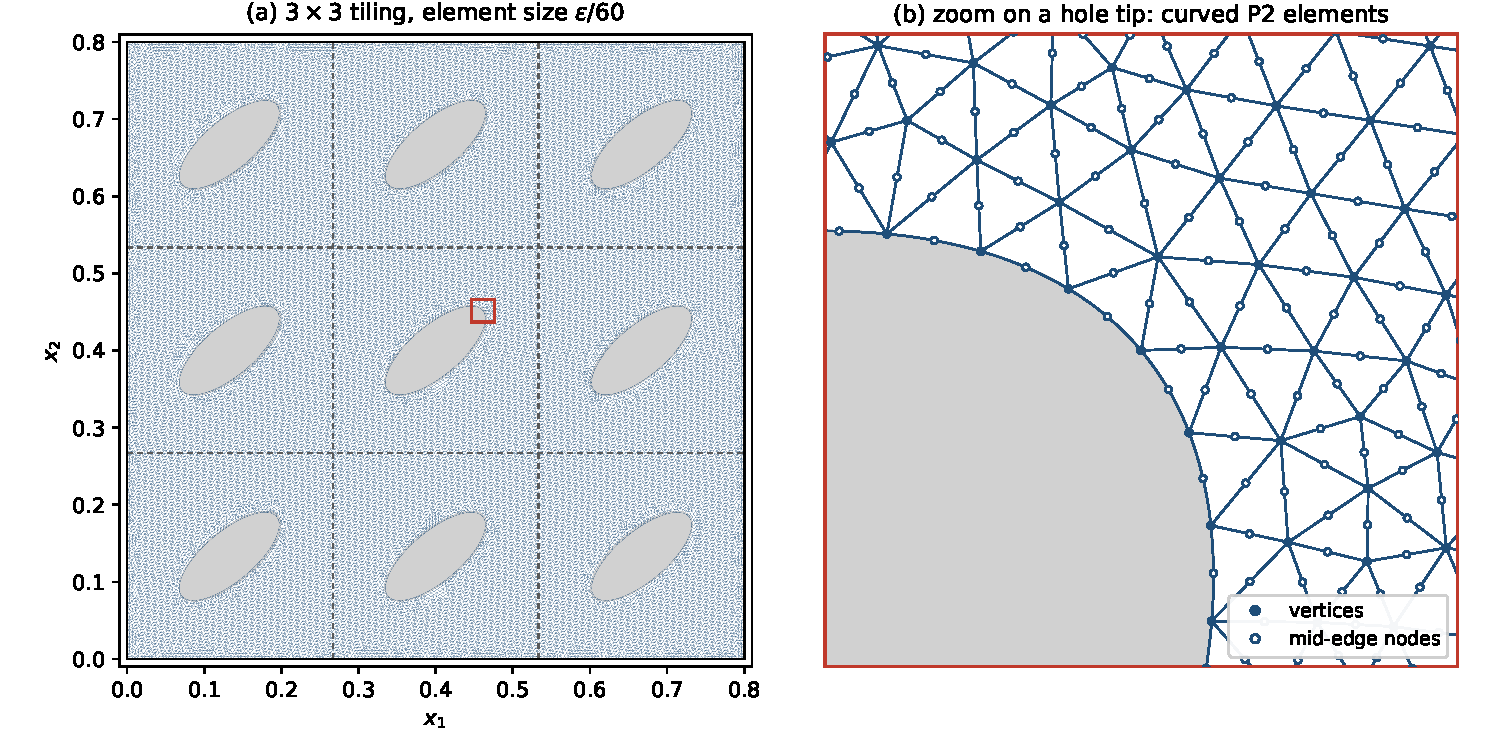
\includegraphics[width=\textwidth]{perforated_rectangle_mesh.pdf}
  \caption{DNS mesh exactly as used in Section~\ref{sec:setup}, for $3\times3$ cells of the
  rotated elliptical hole ($a=0.3$, $b=0.12$, $40^{\circ}$) on $[0,0.8]^2$, with
  second-order triangles of size $\varepsilon/60$, the finest of the three mesh levels
  of the convergence study. (a) The whole plate, with the cell boundaries dashed; at
  this resolution the individual elements are barely visible. (b) Close-up of the region
  framed in (a), at the tip of a hole, where each edge of the six-node triangles is
  drawn as the quadratic curve through its mid-edge node, so that the edges lying on
  the hole follow its boundary instead of cutting across it. Generated by
  \texttt{scripts/06\_mesh\_figure.py}.}
  \label{fig:perforated_rectangle}
\end{figure}

\FloatBarrier
\subsubsection{DNS - discussion}
\label{sec:dns_discussion}

The main difficulty involved in the direct numerical solve is that a geometry
with dense perforations must be constructed and meshed. Since the holes must
be resolved individually, the mesh has to be locally refined around each
inclusion; as the number of inclusions grows, so does the total element
count, roughly in proportion to the number of holes for a fixed
resolution-per-hole. Beyond a modest number of perforations the resulting
linear system becomes prohibitively large, and the simulation fails to
terminate within a practical time frame. Compounding this, the geometry
construction step itself (building and meshing hundreds of small circular
cutouts in \texttt{gmsh}) becomes increasingly slow and fragile, independently
of the linear solve. These two difficulties -- geometric complexity and
system size -- are precisely what motivate the homogenization approach
introduced next: the microstructure is replaced by an equivalent smooth
material, so that the expensive fine geometry only ever needs to be resolved
once, on a single small unit cell, rather than once per macroscopic problem.

\FloatBarrier
\section{Homogenization }

The DNS approach discussed above solves the exact problem at the cost of
resolving every inclusion explicitly. Homogenization instead asks: viewed
from far enough away that individual holes are no longer visible, what
effective, hole-free material would produce the same macroscopic
temperature field? If such an equivalent material can be found, the
macroscopic problem can be solved on a plain, coarse mesh with no
microstructure to resolve at all, at a fraction of the DNS cost. This section
develops that idea: first defining the effective conductivity tensor that
characterizes the equivalent material, then deriving how it is computed from
a single small unit-cell problem, and finally showing how the fine-scale
temperature field can be reconstructed from the coarse solution without ever
meshing the real, perforated domain.

\FloatBarrier
\subsection{Effective conductivity tensor }
\label{sec:effective}

The effective conductivity tensor $\kappa^{\star}$ is the conductivity of the
fictitious, homogeneous material that reproduces the same macroscopic
behaviour as the true, perforated medium, once microscopic fluctuations have
been averaged out. Formally, if $T (x)$ denotes the macroscopic
temperature field (the local cell-average of the true, fine-scale temperature
$u$) and $q$ the macroscopic heat flux, the two are related by the
constitutive law
\begin{equation}
  \label{eq:constitutive}
  q = - \kappa^{\star} \nabla T
\end{equation}
A tensor, rather than a single scalar, is required in general because a
perforated medium need not conduct equally well in every direction: an
elongated or rotated inclusion can make the material conduct more readily
along one axis than another, and can even deflect flux sideways relative to
the imposed gradient. The diagonal entries $\kappa^{\star}_{11},
\kappa^{\star}_{22}$ describe conduction in directions $1$ and $2$ respectively; the
off-diagonal entries $\kappa^{\star}_{12} = \kappa^{\star}_{21}$ (symmetry is
discussed below) describe this cross-direction coupling, and vanish whenever
the microstructure possesses the appropriate mirror symmetries (e.g. a
circular or axis-aligned elliptical inclusion). We are interested in
$\kappa^{\star}$ in this study both because it is the object that makes the
macroscopic problem solvable without resolving the microstructure, and
because it provides a compact, coordinate-free summary of how a given
inclusion shape affects heat transport -- the central question this study
sets out to explore.

\FloatBarrier
\subsubsection{Computing the effective conductivity}
\label{sec:cell_problem}

Two length scales coexist in the perforated plate, and the notation keeps them
apart. Positions in the plate are given by the macroscopic coordinate
$x = (x_1, x_2) \in \Omega$. If $\varepsilon$ is the side length of one periodic
cell, rescaling a single cell and its inclusion to unit size gives the unit
cell $Y = [0, 1]^2$, in which positions are given by the microscopic coordinate
$y = (y_1, y_2) \in Y$. A point $x$ of the plate thus sits at the position
$y = \{ x / \varepsilon \}$ within its own cell, where $\{ \cdot \}$ denotes the
fractional part taken componentwise. We write $Y_{\tmop{solid}}$ for the unit
cell with the inclusion removed, $\nabla_y$ for the gradient with respect to
$y$, and $e_1, e_2$ for the unit vectors of the two coordinate directions,
which are simply called directions $1$ and $2$ from now on. The two coordinates
and the correspondence between them are sketched in Fig.~\ref{fig:bc_cell}(a).

The effective tensor is obtained from two auxiliary problems posed on the unit
cell alone, one for each direction. For $j \in \{ 1, 2 \}$, the corrector
$\chi_j$ is the function on $Y_{\tmop{solid}}$ that solves
\begin{equation}
  \label{eq:cell_problem}
  \left\{ \begin{array}{ll}
    \nabla_y \cdot \left( \kappa \left( e_j + \nabla_y \chi_j \right) \right) = 0
    & \tmop{in} Y_{\tmop{solid}}\\
    \kappa \left( e_j + \nabla_y \chi_j \right) \cdot \mathbf{n} = 0 & \tmop{on}
    \tmop{the} \tmop{inclusion} \tmop{wall}\\
    \chi_j (0, y_2) = \chi_j (1, y_2), \quad \chi_j (y_1, 0) = \chi_j (y_1, 1) &
    \forall y_1, y_2 \in [0, 1]\\
    \displaystyle\int_{Y_{\tmop{solid}}} \chi_j \, dy = 0 &
  \end{array} \right.
\end{equation}
The third condition makes $\chi_j$ periodic on the cell. The first three
conditions determine $\chi_j$ only up to an additive constant, since adding a
constant changes neither its gradient nor its periodicity, and the zero-mean
condition removes this freedom so that the solution is unique. It is also the
natural normalization, consistent with $T$ being the average of the fine-scale
temperature over a cell. Figure~\ref{fig:bc_cell}(b) shows on which part of the cell
boundary each of the other conditions applies.

\begin{figure}[h]
  \centering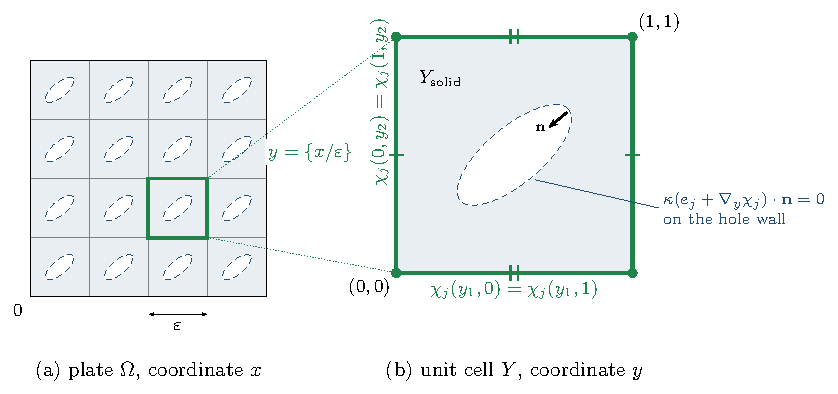
\includegraphics[width=0.95\textwidth]{bc_cell.pdf}
  \caption{The two coordinates and the cell problem. (a) The plate is a tiling of cells of
  side $\varepsilon$, and the fractional part $y=\{x/\varepsilon\}$ maps every one
  of them onto the same unit cell. (b) The boundary conditions of the cell problem
  of Eq.~\eqref{eq:cell_problem}. The corrector takes equal values on the left and
  right faces and on the bottom and top faces, the faces being paired by the
  single and double tick marks, while the hole wall is insulated. The four corners,
  marked by dots, are all tied to $(0,0)$ in the discrete problem.}
  \label{fig:bc_cell}
\end{figure}

The meaning of the correctors is clearest through the functions
\[ t_j (y) = y_j + \chi_j (y), \qquad j \in \{ 1, 2 \} . \]
Since $\nabla_y t_j = e_j + \nabla_y \chi_j$, Eq.~\eqref{eq:cell_problem} states that
$t_j$ is a steady temperature field in the solid part of the cell, insulated on
the inclusion wall, whose values on opposite faces differ by exactly one in
direction $j$ and coincide in the other direction. In other words, $t_j$ is the
temperature of a cell subjected to a unit macroscopic gradient $e_j$. Without
the inclusion it would be the linear profile $y_j$, and the corrector $\chi_j$
is precisely the small periodic deviation from this profile that the
inclusion forces as heat is diverted around it, vanishing identically when
there is no hole.

Multiplying by a periodic test function and integrating by parts as in
Section~\ref{sec:application} gives the weak form solved in practice, in which
the boundary terms vanish because the contributions of opposite faces cancel
by periodicity and no heat crosses the inclusion wall. It reads: find $\chi_j$,
periodic on $Y$ with zero mean, such that
\begin{equation}
  \label{eq:cell_weak}
  \int_{Y_{\tmop{solid}}} \kappa \nabla_y \chi_j \cdot \nabla_y v \; dy = -
  \int_{Y_{\tmop{solid}}} \kappa e_j \cdot \nabla_y v \; dy \quad \forall v \;
  Y\tmop{-periodic} .
\end{equation}
The effective tensor is then the average, over the whole cell, of the local
heat flux produced by a unit gradient in direction $j$,
\begin{equation}
  \label{eq:Kstar}
  \kappa^{\star}_{ij} = \frac{1}{| Y |} \int_{Y_{\tmop{solid}}} \kappa \left(
  e_j + \nabla_y \chi_j \right) \cdot e_i \; dy = \frac{1}{| Y |}
  \int_{Y_{\tmop{solid}}} \kappa \frac{\partial t_j}{\partial y_i} \; dy ,
\end{equation}
so that its $j$-th column is the mean flux carried by a cell subjected to the
gradient $e_j$. The normalization uses the area $| Y |$ of the full cell,
inclusion included, rather than the solid area alone, and this is what
accounts for the loss of conductivity due to porosity. Taking $v = \chi_i$ in
Eq.~\eqref{eq:cell_weak} shows that 
$$\int_{Y_{\tmop{solid}}} \kappa (e_j +
\nabla_y \chi_j) \cdot \nabla_y \chi_i \, dy = 0$$ 
which turns
Eq.~\eqref{eq:Kstar} into
\[ \kappa^{\star}_{ij} = \frac{1}{| Y |} \int_{Y_{\tmop{solid}}} \kappa \nabla_y
   t_i \cdot \nabla_y t_j \; dy . \]
This form is manifestly symmetric in $i$ and $j$, so $\kappa^{\star}$ is
symmetric whenever the local conductivity $\kappa$ is, which here, $\kappa$
being a scalar, is always the case. The property is used throughout this study
as a check on the implementation.

In practice the two cell problems are solved once per inclusion shape, on a
mesh of the unit cell only, which can therefore afford a high resolution.
Periodicity is enforced both on the mesh, whose nodes are placed identically on
opposite faces, and on the linear system, in which each degree of freedom on
the right face is tied to its image on the left face and each on the top face
to its image on the bottom. The three corners $(1, 0)$, $(0, 1)$ and $(1, 1)$,
marked in Fig.~\ref{fig:bc_cell}(b),
are tied directly to $(0, 0)$, since the corner $(1, 1)$ would otherwise be
constrained twice and the computed corrector could jump across the faces near
it. The zero-mean condition is imposed in two stages, by pinning one degree of
freedom to remove the additive constant during the solve and shifting the
result to zero mean afterwards. The resulting system is small and is solved
with a direct LU solver, which gives $\kappa^{\star}_{12} = \kappa^{\star}_{21}$
to machine precision.

\FloatBarrier
\subsubsection{Effective conductivity and perforation shapes}

Figure~\ref{fig:cell_fields} shows the temperature field obtained from a single
unit cell problem, together with the local heat flux, for a circular and an
elliptical inclusion, and Figs.~\ref{fig:temp_circle} and~\ref{fig:temp_ellipse},
in the appendix, show the corresponding fields over a whole perforated plate. In both cases
the flux visibly bends around the inclusion, as the zero-flux condition of
Eq.~\eqref{eq:cell_problem} requires, since no heat can cross into the hole and
the flux must therefore remain tangent to its boundary. For the circular
inclusion the resulting tensor is isotropic and diagonal to within numerical
precision, with $\kappa^{\star}_{11} = \kappa^{\star}_{22}$ and
$\kappa^{\star}_{12} = 0$, as expected from the four-fold rotational symmetry of a
circle in a square cell. No direction is geometrically preferred, so none can
be preferred by the effective conductivity either.

\begin{figure}[h]
  \centering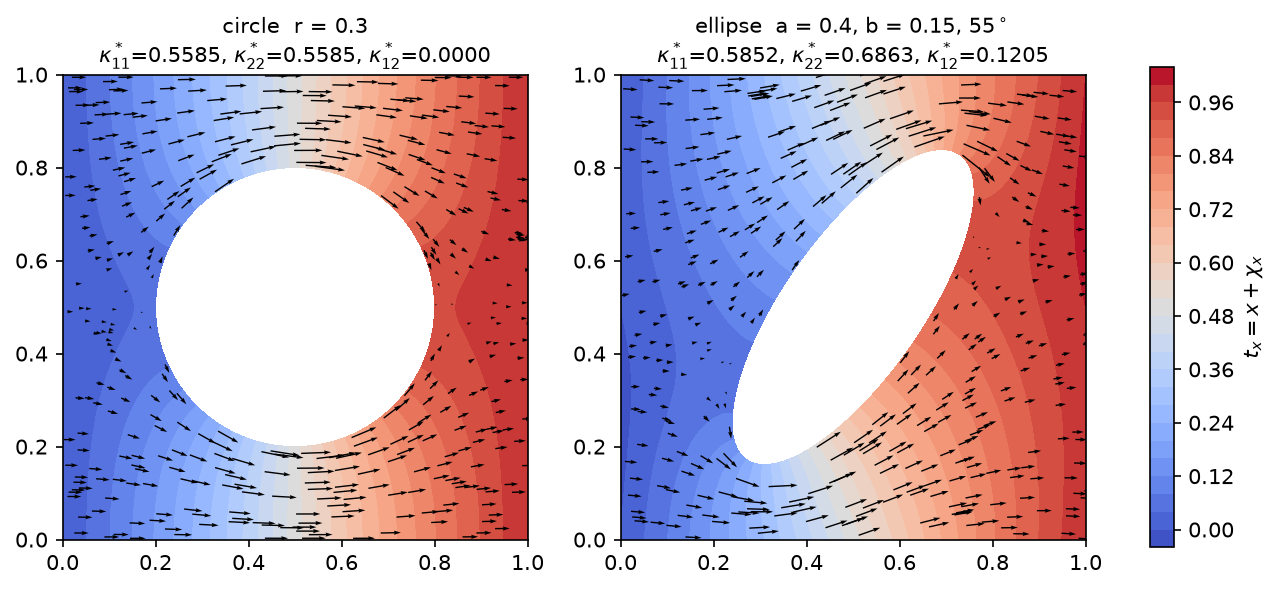
\includegraphics[width=\textwidth]{cell_fields.png}
  \caption{Unit-cell solution for a unit gradient in direction $1$: local temperature
  $t_1 = y_1 + \chi_1$ (colour) and heat flux (arrows) for the circular and
  elliptical inclusions. The flux is tangent to the hole wall and squeezes
  through the narrow gaps; for the tilted ellipse it is deflected off-axis,
  which is what the non-zero $\kappa^{\star}_{12}$ records. Generated by
  \texttt{scripts/03\_cell\_fields.py}.}
  \label{fig:cell_fields}
\end{figure}

Elongating the inclusion into an ellipse breaks this symmetry and makes the
anisotropy directly visible. Done naively, elongation changes two things at
once, because at fixed semi-axis $a$ a thinner ellipse is also a smaller hole,
which lowers the porosity and lets every direction conduct better. To isolate
the effect of shape, Fig.~\ref{fig:ellipse_sweeps}(a) varies the aspect ratio $b/a$
of an axis-aligned ellipse at constant hole area $ab = 0.06$, that is, at
constant porosity. The expected trade-off then appears cleanly. Heat is
increasingly free to travel along the elongated axis, so that $\kappa^{\star}_{11}$
rises, and increasingly obstructed across it, so that $\kappa^{\star}_{22}$ falls,
steeply so once the gap between neighbouring holes becomes narrow. The trade-off is far
from symmetric, as over the range shown $\kappa^{\star}_{22}$ loses about three times as
much as $\kappa^{\star}_{11}$ gains.

\begin{figure}[h]
  \centering
  \begin{minipage}{0.49\textwidth}\centering
    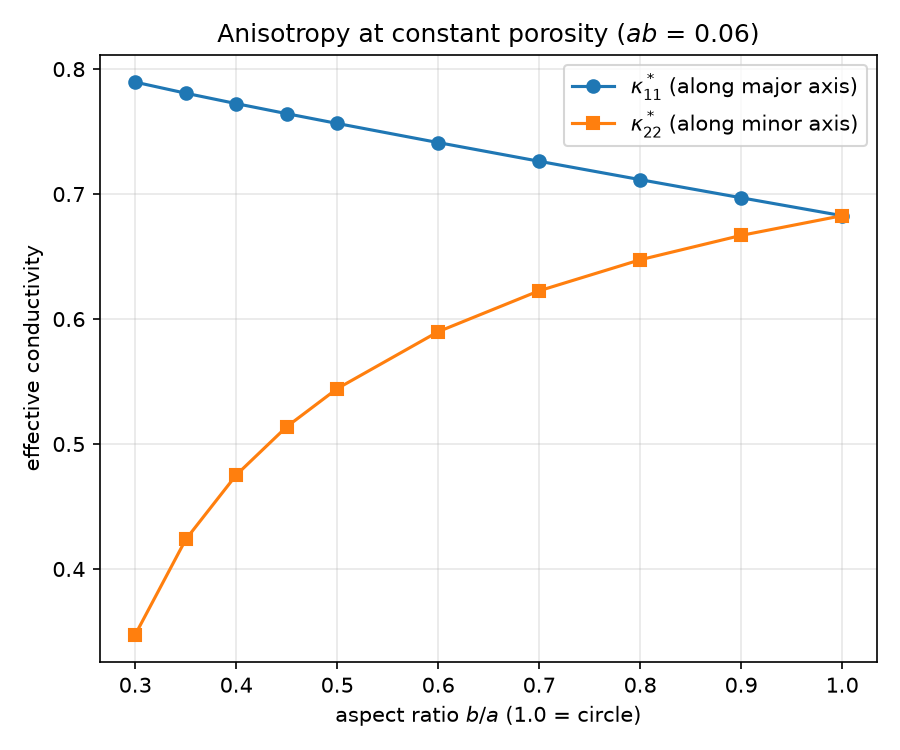
\includegraphics[width=\textwidth]{ellipse_aspect_sweep.png}\\ (a)
  \end{minipage}\hfill
  \begin{minipage}{0.49\textwidth}\centering
    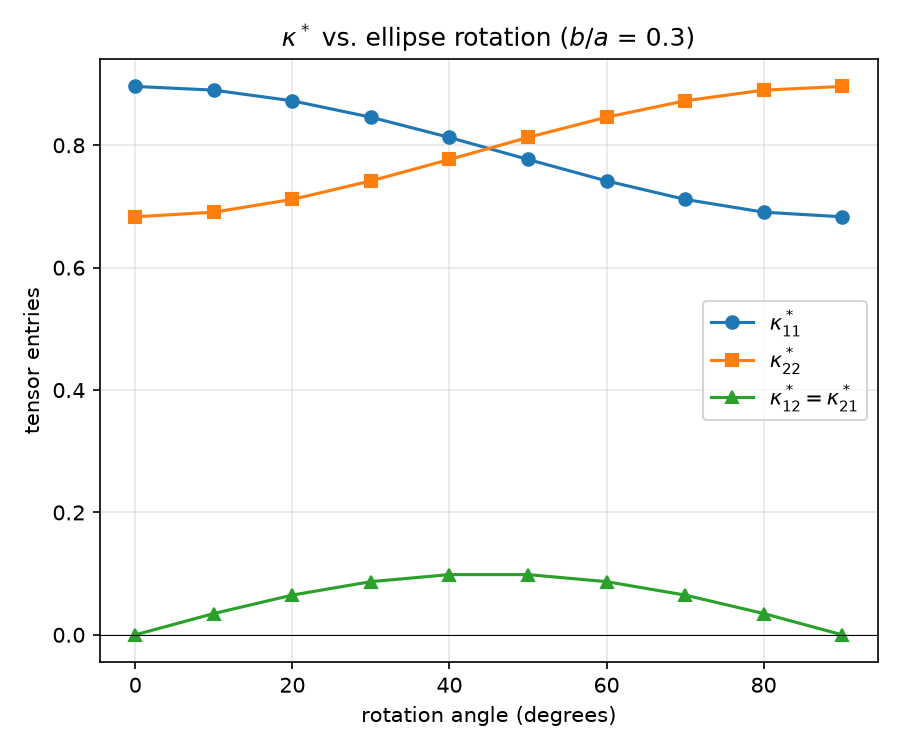
\includegraphics[width=\textwidth]{ellipse_rotation_sweep.png}\\ (b)
  \end{minipage}
  \caption{Effective conductivity tensor of an elliptical hole as its shape
  changes. (a) Entries $\kappa^{\star}_{11}$ and $\kappa^{\star}_{22}$ of an
  axis-aligned ellipse as a function of its aspect ratio $b/a$, at constant hole
  area $ab = 0.06$ and hence constant porosity, $b/a = 1$ being a circle.
  $\kappa^{\star}_{11}$ rises and $\kappa^{\star}_{22}$ falls as the ellipse is
  elongated in direction $1$. (b) The three independent entries as a function of
  the rotation angle of the ellipse, at the fixed aspect ratio $b/a = 0.3$ with
  $a = 0.3$. Rotating the ellipse away from the coordinate axes generates a non-zero
  off-diagonal entry, as the imposed gradient is increasingly deflected off-axis by
  the tilted inclusion. Generated by \texttt{scripts/02\_ellipse\_sweeps.py}.}
  \label{fig:ellipse_sweeps}
\end{figure}

An axis-aligned ellipse still possesses mirror symmetry about both coordinate
axes, however, so $\kappa^{\star}_{12}$ remains zero whatever its aspect ratio,
and breaking this remaining symmetry requires rotating the ellipse.
Figure~\ref{fig:ellipse_sweeps}(b) follows the three independent entries of
$\kappa^{\star}$ as a fixed, elongated ellipse is rotated from $0^{\circ}$ to
$90^{\circ}$. The off-diagonal entry vanishes at the two axis-aligned extremes
and is largest near $45^{\circ}$, where the principal axis of the inclusion is
furthest from both coordinate directions. Physically, this is the tensor's way
of recording that a macroscopic gradient imposed purely in direction $1$ now
produces a flux with a genuine component in direction $2$, the tilted inclusion
deflecting heat sideways. The sweep also reflects the symmetry of the square
cell, since rotations by $\theta$ and by $90^{\circ} - \theta$ give mirror-image
holes, for which $\kappa^{\star}_{11}$ and $\kappa^{\star}_{22}$ swap while
$\kappa^{\star}_{12}$ is unchanged. Throughout, the measured asymmetry
$| \kappa^{\star}_{12} - \kappa^{\star}_{21} |$ stays at the level of machine
precision, around $10^{-15}$, as the symmetry argument above requires.

\FloatBarrier
\subsection{First order approximation}

Section~\ref{sec:effective} obtained the effective tensor $\kappa^{\star}$ from a
single, cheap unit-cell computation. This subsection uses it to solve the
macroscopic problem without ever meshing the perforated domain, and then
recovers the fine-scale temperature from the coarse solution.

\FloatBarrier
\subsubsection{Macroscopic problem and fine-scale reconstruction}
\label{sec:reconstruction}

With $\kappa^{\star}$ in hand, the macroscopic temperature $T$ solves the
homogeneous, hole-free problem
\begin{equation}
  \label{eq:macro_problem}
  \left\{ \begin{array}{c}
    \nabla \cdot \left( \kappa^{\star} \nabla T \right) = 0, \quad \tmop{on}
    \Omega \\
    \tmop{same} \tmop{Dirichlet}/\tmop{Neumann} \tmop{boundary} \tmop{conditions}
    \tmop{as} \tmop{Eq.}~\eqref{eq:bc}
  \end{array} \right.
\end{equation}
on the macroscopic domain $\Omega$, meshed as a plain rectangle without a
single inclusion and sketched in Fig.~\ref{fig:bc_dns}(b). On the insulated top and
bottom edges the zero-flux condition now reads $(\kappa^{\star}\nabla T)\cdot\mathbf{n}=0$,
the flux being given by the constitutive law of Eq.~\eqref{eq:constitutive}. This is the DNS problem of Eq.~\eqref{eq:heat_steady}
with the scalar conductivity $\kappa$ replaced by the constant and generally
anisotropic tensor $\kappa^{\star}$, and since nothing small remains to be
resolved, a coarse mesh suffices.

The fine-scale temperature is then expressed in terms of $T$ and the
correctors by the two-scale expansion
\begin{equation}
  \label{eq:twoscale_ansatz}
  u^{\varepsilon} (x) = T (x) + \varepsilon \sum_{j = 1}^2 \chi_j \left( \left\{
  \frac{x}{\varepsilon} \right\} \right) \frac{\partial T}{\partial x_j} (x) + O
  (\varepsilon^2),
\end{equation}
whose first two terms we abbreviate as $T + \varepsilon \chi \cdot \nabla T$, with
$\chi = (\chi_1, \chi_2)$. The remainder is the theoretical error of the method.
Away from the boundary of $\Omega$, near which the expansion breaks down for
reasons discussed below, homogenization theory predicts that the
first neglected term is of order $\varepsilon^2$, so that the reconstruction
$T + \varepsilon \chi \cdot \nabla T$ approximates the fine-scale temperature to
second order in $\varepsilon$, whereas $T$ alone, which ignores the oscillation
that the holes imprint on the temperature, is only accurate to first order.
Verifying these two rates is the main purpose of Section~\ref{sec:results}.

Evaluating the reconstruction at a point $x$ requires $T$ and its gradient at
$x$, read off the coarse macroscopic solution, and the correctors at the
position $y = \{ x / \varepsilon \}$ of $x$ within its cell. Because the
correctors are periodic and were computed once on the unit cell, this single
small computation stands in for every cell of the plate, and no mesh of the
full microstructure is ever built. The reconstruction is an explicit formula
rather than a further PDE, so it can be evaluated at as many points as
desired, along a line, on a grid for visualization or at the sampling points
of a DNS comparison, at negligible cost.

\FloatBarrier
\subsubsection{Algorithm}
\label{sec:algorithm}

The full homogenization pipeline implemented in this study consists of the
following steps.
\begin{enumeratenumeric}
  \item \textbf{Cell problem.} Mesh the unit cell $Y$ with the desired
  inclusion, registering periodicity on opposite faces, and solve the two cell
  problems of Eq.~\eqref{eq:cell_weak}, one per direction, normalizing each
  corrector to zero mean.
  
  \item \textbf{Effective tensor.} Assemble the $2 \times 2$ tensor
  $\kappa^{\star}$ from the two correctors via Eq.~\eqref{eq:Kstar}.
  
  \item \textbf{Macroscopic solve.} Mesh the macroscopic domain $\Omega$ coarsely,
  without any microstructure, and solve Eq.~\eqref{eq:macro_problem} for $T$
  with the constant tensor obtained in step 2.
  
  \item \textbf{Reconstruction.} Wherever the fine-scale temperature is needed,
  evaluate $T + \varepsilon \chi \cdot \nabla T$ using $T$ and its gradient from
  step 3 and the correctors from step 1.
\end{enumeratenumeric}
The gain over the DNS of Section~\ref{sec:dns_discussion} comes from a clean
separation of scales. Step 1 is the only step in which the microstructure is
meshed, and it is solved once, on a mesh containing a single inclusion,
however large or complex the macroscopic domain may be. Step 3 is a coarse
solve on a hole-free mesh and step 4 is the pointwise evaluation of an explicit
formula, so the cost of both is essentially independent of $\varepsilon$. Packing
more and smaller cells into the same domain leaves the macroscopic mesh
unchanged, whereas the cost of the DNS grows sharply with the number of
inclusions it must resolve. The one-time cost of step 1 is amortized further
whenever $\kappa^{\star}$ is reused for other domain shapes, boundary conditions
or load cases, none of which require solving the cell problem again.

\FloatBarrier
\subsubsection{Validation setup}
\label{sec:setup}

The homogenization pipeline was validated against a DNS on a geometry built so that
the two are directly comparable. The DNS domain is an exact tiling of the unit cell used
in the corrector problems, with the same hole shape and size relative to the cell and the
cells arranged edge to edge without margins, so that the DNS and the homogenized model
describe, by construction, the same material. The domain is the square $[0, L]^2$ with
$L = 0.8$, divided into $n \times n$ cells of size $\varepsilon = L / n$ with $n$ from $2$
to $12$, and every solve, whether of the cell problem, the macroscopic problem or the DNS,
uses P2 elements on curved meshes as described in Section~\ref{sec:p2}.

\paragraph{Choice of hole.} A circular hole cannot show the homogenization
error with the boundary conditions of Eq.~\eqref{eq:bc}. For a centred circle,
$\kappa^{\star}$ is isotropic, so the macroscopic solution is the linear profile
$T = x_1 / L$, and the mirror symmetries of the cell make $\chi_1$ vanish on the cell
faces $y_1 = 0, 1$ and $\partial \chi_1 / \partial y_2$ vanish on $y_2 = 0, 1$. The reconstruction
$x_1/L + (\varepsilon / L)\, \chi_1(\{x/\varepsilon\})$ then satisfies the heat
equation, the insulated hole walls, both Dirichlet conditions and the insulated
top and bottom edges. It is thus the exact solution of the DNS problem, and
any measured difference is FEM error. We therefore use a rotated ellipse,
$a = 0.3$, $b = 0.12$, rotated by $40^{\circ}$, for which
\[
\kappa^{\star} \approx \begin{pmatrix} 0.78 & 0.09 \\ 0.09 & 0.75 \end{pmatrix}.
\]
Because $\kappa^{\star}_{12} \neq 0$, the insulated top and bottom edges now
require $\kappa^{\star}_{21} \partial T / \partial x_1 + \kappa^{\star}_{22} \partial T / \partial x_2 = 0$, so $T$
is no longer linear and the two-scale expansion has a genuine error.

\FloatBarrier
\subsubsection{Boundary layers}
\label{sec:boundary_layer}

The two-scale expansion of Eq.~\eqref{eq:twoscale_ansatz} is built from correctors
that only know about the periodic cell, and nothing in its construction refers to the
boundary of $\Omega$. Away from the boundary this does no harm, but on $\partial\Omega$
the reconstruction does not in general satisfy the boundary conditions, and the true
solution has to make up the difference within a thin region along the boundary, called
a boundary layer. This subsection introduces the finite-sample problem in which the layer is easiest
to see, explains why the layer appears, measures how thick it is, and uses this
measurement to predict how the conductivity measured on a finite sample converges to
$\kappa^{\star}$.

\paragraph{A finite sample.} Besides the field comparison based on Eq.~\eqref{eq:bc},
this study measures the conductivity tensor of a finite perforated sample and compares it
with $\kappa^{\star}$. The sample is the $n \times n$ tiling of Section~\ref{sec:setup}, on
which the DNS is solved twice, with the affine temperature $u_j = x_j$ imposed on the whole
outer boundary for $j = 1, 2$ and the hole walls insulated, as sketched in
Fig.~\ref{fig:boundary_layer}. The apparent tensor of the sample is its volume-averaged
flux,
\begin{equation}
  \label{eq:Kapp}
  \kappa^{\mathrm{app}}_{ij} = \frac{1}{|\Omega|} \int_{\Omega_{\mathrm{solid}}} \kappa\, \partial_i u_j \; dx ,
\end{equation}
normalized, like $\kappa^{\star}$, by the full area $|\Omega|$. This affine problem is also
the cleanest setting in which to see the boundary layer.

\paragraph{Why a layer appears.} With the affine data $u = x_j$, the macroscopic
solution is exactly $T = x_j$. The reconstruction
$x_j + \varepsilon \chi_j (\{ x / \varepsilon \})$ has the local gradient
$e_j + \nabla_y \chi_j$, and by Eq.~\eqref{eq:cell_problem} it therefore satisfies the
heat equation in the solid and the insulation condition on every hole wall exactly. Its
only defect lies on the outer boundary, where it exceeds the imposed data by
$\varepsilon \chi_j (\{ x / \varepsilon \})$. Writing the true solution as
\begin{equation}
  \label{eq:layer_split}
  u^{\varepsilon} (x) = x_j + \varepsilon \chi_j \left( \left\{ \frac{x}{\varepsilon}
  \right\} \right) + \varepsilon \theta (x),
\end{equation}
the correction $\theta$ solves the same perforated problem as $u^{\varepsilon}$, with the
boundary data $\theta = - \chi_j (\{ x / \varepsilon \})$ on $\partial \Omega$. Since this
data oscillates on the scale of a cell, one expects the correction to be felt only near
the boundary, and the question is how far into the plate it reaches.

\begin{figure}[h]
  \centering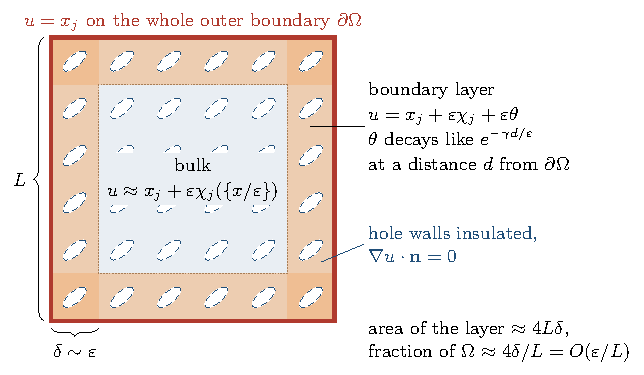
\includegraphics[width=0.95\textwidth]{boundary_layer.pdf}
  \caption{Boundary layer of a finite perforated sample on which the affine temperature
  $u=x_j$ is imposed along the whole outer boundary, the hole walls being
  insulated, which is the setting of Eq.~\eqref{eq:Kapp}. In the bulk the solution
  is the two-scale expansion $x_j+\varepsilon\chi_j$, which however does not match
  the boundary data. The correction $\varepsilon\theta$ that restores it decays
  exponentially with the distance $d$ to the boundary over a length proportional
  to $\varepsilon$, so that it is confined to a band of thickness $\delta\sim\varepsilon$
  covering an area of about $4L\delta$, a fraction $4\delta/L=O(\varepsilon/L)$ of the
  sample.}
  \label{fig:boundary_layer}
\end{figure}

\paragraph{Measuring the layer.} This question is answered numerically in
Fig.~\ref{fig:boundary_layer_profile}, for the rotated elliptical hole of
Section~\ref{sec:setup} and $u = x_1$ imposed on the whole outer boundary. Because the
expansion is exact away from the boundary for this boundary data, the difference between
the DNS and $x_1 + \varepsilon \chi_1$ is the correction $\varepsilon \theta$ alone, and
its map in Fig.~\ref{fig:boundary_layer_profile}(a) is indeed confined to a narrow band
along the boundary. To see how thick this band is, the difference is averaged over thin
strips parallel to the boundary and plotted against the distance $d$ to the boundary,
measured in cells, that is $d / \varepsilon$, which gives the profiles of
Fig.~\ref{fig:boundary_layer_profile}(b). Two observations stand out.

First, the profiles obtained for $n = 4$, $8$ and $12$ fall on a single curve. Measured in
cells, the layer therefore looks the same whatever the cell size, which means that
$\theta$ depends on $x$ only through $x / \varepsilon$, and in physical units its
thickness is proportional to $\varepsilon$. The opposite edges lie $4$ cells away in the
first case and $12$ in the last, so the agreement also shows that each edge produces its
own layer, unaffected by the others.

Second, this common curve is a straight line on the logarithmic scale, so the layer
decays exponentially with the distance to the boundary,
\begin{equation}
  \label{eq:layer_decay}
  \varepsilon \, | \theta | \propto \varepsilon \, e^{- \gamma d / \varepsilon},
\end{equation}
with a fitted rate $\gamma = 5.65$. The layer thus loses a factor ten every
$0.41 \varepsilon$, and a little under one cell from the boundary it has fallen by more
than two orders of magnitude and disappears below the discretization error. Further from
the boundary nothing is left of it, the mean of $\theta$ beyond one and a half cells being
of order $10^{-8}$.

The same mechanism is at work in the problem of Eq.~\eqref{eq:bc}, where on the Dirichlet
edges the reconstruction misses the imposed temperature by
$\varepsilon \chi \cdot \nabla T$, and on the insulated edges the flux of the
reconstruction vanishes only on average along each cell. This is why the field
errors are best measured at a distance from the edges.

\begin{figure}[h]
  \centering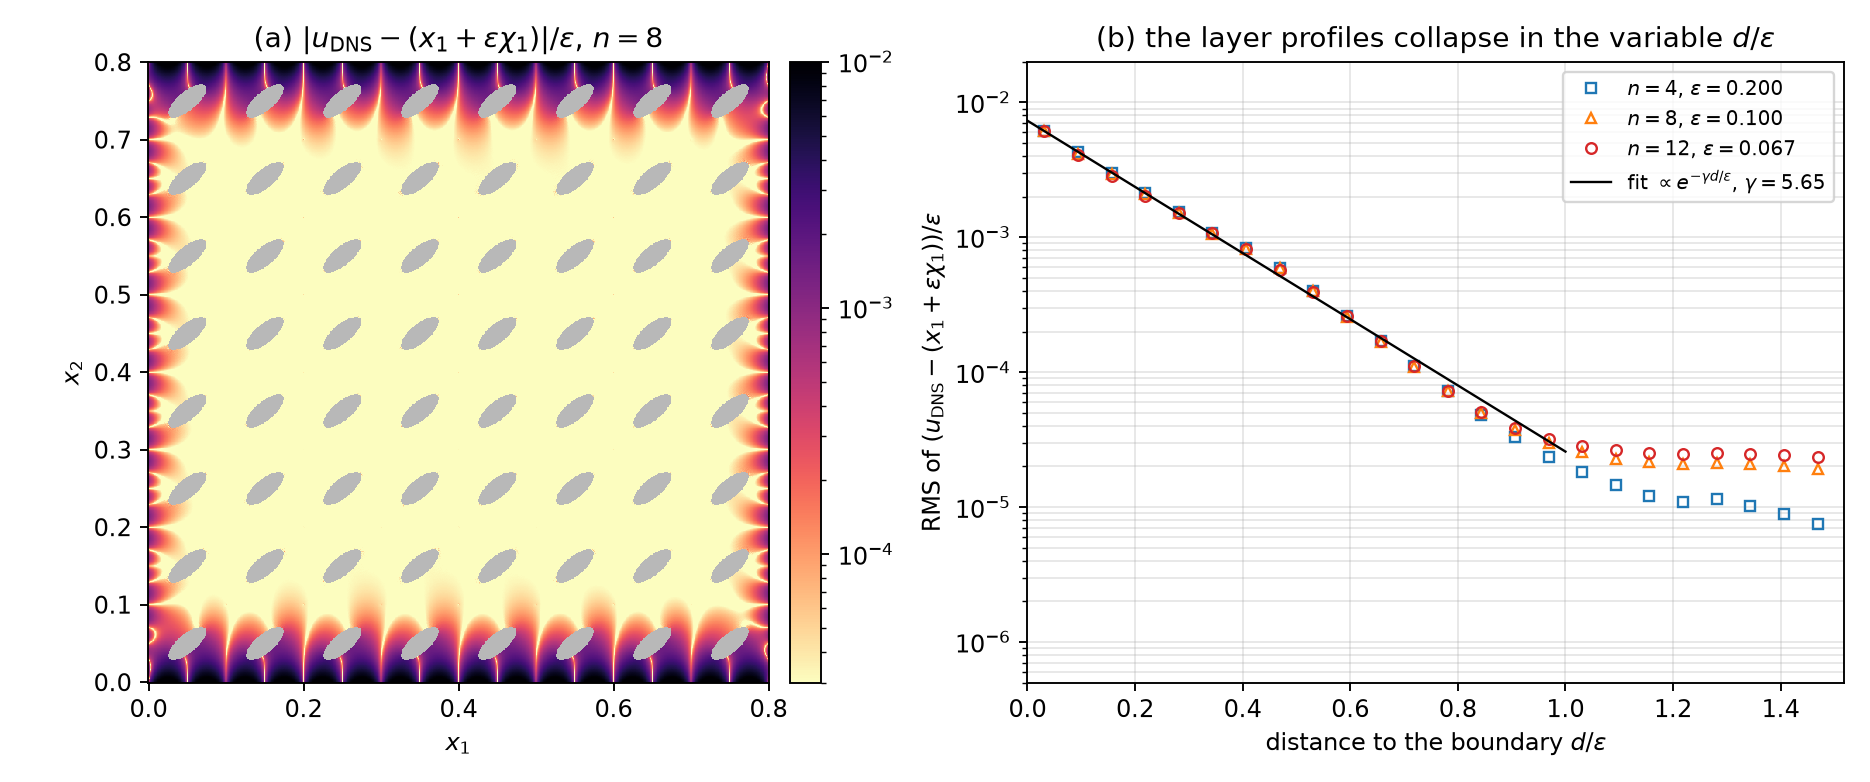
\includegraphics[width=\textwidth]{boundary_layer_profile.png}
  \caption{Measured boundary layer for the rotated ellipse ($a=0.3$, $b=0.12$, $40^{\circ}$),
  with $u=x_1$ imposed on the whole outer boundary. Since the expansion
  $x_1+\varepsilon\chi_1$ is exact in the bulk for this boundary data, its difference
  with the DNS is the boundary layer alone. (a) Map of this difference, divided by
  $\varepsilon$, for $n=8$, on a logarithmic scale with the holes in grey. (b) Its RMS
  over strips of width $\varepsilon/16$ parallel to the boundary, against the distance
  to the boundary in units of $\varepsilon$, for three cell sizes. The three profiles
  coincide, which shows that the layer depends on $x$ only through $x/\varepsilon$, and
  decay exponentially at the fitted rate $\gamma=5.65$ until they reach the level of the discretization error a little
  under one cell from the boundary. Generated by
  \texttt{scripts/07\_boundary\_layer.py}.}
  \label{fig:boundary_layer_profile}
\end{figure}

\paragraph{Consequence for the conductivity tensor.} Inserting the decomposition of
Eq.~\eqref{eq:layer_split} into the apparent tensor of Eq.~\eqref{eq:Kapp} splits this
average in two. The first part is the flux of
$x_j + \varepsilon \chi_j (\{ x / \varepsilon \})$, whose gradient
$e_j + \nabla_y \chi_j$ is the same field in every cell. Its average over one cell is
$\kappa^{\star}_{ij}$ by the definition of Eq.~\eqref{eq:Kstar}, and since the sample is
made of a whole number of cells, its average over the sample is exactly
$\kappa^{\star}_{ij}$. This is where the exact tiling matters, as partial cells along the
edges would leave an additional error. What remains is the flux of the layer alone,
\begin{equation}
  \label{eq:Kapp_layer}
  \kappa^{\mathrm{app}}_{ij} - \kappa^{\star}_{ij} = \frac{1}{| \Omega |}
  \int_{\Omega_{\tmop{solid}}} \kappa \, \frac{\partial (\varepsilon \theta_j)}{\partial
  x_i} \, dx,
\end{equation}
where $\theta_j$ is the correction of Eq.~\eqref{eq:layer_split} for the direction $j$.

The two observations above are all that is needed to estimate this integral. By the
first, the layer near a given edge can be written as
$\varepsilon \theta_j (x) = \varepsilon \Theta_j (x / \varepsilon)$, with a profile
$\Theta_j$ that does not depend on $\varepsilon$, and by the second this profile vanishes
beyond about one cell. The chain rule gives
$\partial_{x_i} (\varepsilon \theta_j) = \partial_{y_i} \Theta_j$ with $y = x / \varepsilon$,
the factor $\varepsilon$ in front cancelling the factor $1 / \varepsilon$ produced by the
differentiation. The gradient of the layer is therefore of order one, but it only lives
within a distance of order $\varepsilon$ from the boundary. Along the left edge, changing
variables with $dx = \varepsilon^2 \, dy$, the contribution of the layer to the integral
is
\[ \varepsilon^2 \int \kappa \, \partial_{y_i} \Theta_j \; dy = \varepsilon^2 \cdot
   \frac{L}{\varepsilon} \cdot c_{ij} = \varepsilon L \, c_{ij}, \]
where $L / \varepsilon$ is the number of cells along the edge and $c_{ij}$ is the
contribution of a single cell of the layer, which, like $\Theta_j$, does not depend on
$\varepsilon$. Each of the four edges contributes in this way, with its own constant, and
dividing by $| \Omega | = L^2$ gives
\begin{equation}
  \label{eq:Kapp_rate}
  \kappa^{\mathrm{app}}_{ij} - \kappa^{\star}_{ij} \approx C_{ij} \, \frac{4
  \varepsilon}{L},
\end{equation}
with $C_{ij}$ the average of the four edge constants. In words, a flux error of order one
is spread over a band of width $\delta \sim \varepsilon$ along the boundary, which covers
an area of about $4 L \delta$ and thus a fraction $4 \delta / L = O (\varepsilon / L)$ of
the sample. The only part of the layer this count misses are the four corners, each a
patch of about one cell, which contribute $O (\varepsilon^2 / L^2)$ and are one order
smaller. Equation~\eqref{eq:Kapp_rate} predicts more than the rate $O (\varepsilon)$, since
it says that the ratio of $\kappa^{\mathrm{app}} - \kappa^{\star}$ to
$4 \varepsilon / L$ should be the same number for every $n$, a sharper prediction that can
be checked directly against the measured tensors. The constant itself is small for the
holes studied here, because the layer starts from the small values of $\chi_j$ on the cell
faces and decays within a fraction of a cell.

\FloatBarrier
\subsubsection{Results}
\label{sec:results}

Both comparisons with the DNS use the geometry and the elliptical hole of
Section~\ref{sec:setup}.

\paragraph{Field error: second-order accuracy of the reconstruction.} The DNS field
$u_{\mathrm{DNS}}$ is compared with two approximations, the macroscopic field $T$ alone
and the two-scale reconstruction $T + \varepsilon \chi \cdot \nabla T$ of
Eq.~\eqref{eq:twoscale_ansatz}, on a $40 \times 40$ grid of points covering
$[0.15 L, 0.85 L]^2$, points falling inside a hole being skipped.
Figure~\ref{fig:homogenization_error} shows the RMS of both differences against the cell
size. The macroscopic field alone converges at first order, with a fitted rate
\[
\mathrm{RMS}(u_{\mathrm{DNS}} - T) \sim \varepsilon^{0.97},
\]
which is expected since it misses the oscillation of amplitude $\varepsilon$ that the
holes imprint on the temperature. Adding the corrector restores this oscillation, and
the error of the reconstruction then decays at second order,
\[
\mathrm{RMS}\big(u_{\mathrm{DNS}} - (T + \varepsilon \chi \cdot \nabla T)\big) \sim \varepsilon^{2.02} .
\]
This is the central result of the study, and it is what the expansion of
Eq.~\eqref{eq:twoscale_ansatz} predicts, the first neglected term being of the form
$\varepsilon^2 \chi_{ij}(\{x/\varepsilon\})\, \partial_i \partial_j T$, with second-order
correctors $\chi_{ij}$, which does not vanish here because $T$ is curved. The two rates
open a gap that widens as the cells shrink, and at the smallest cell size the
reconstruction is about two hundred times more accurate than $T$ alone.

\begin{figure}[h]
  \centering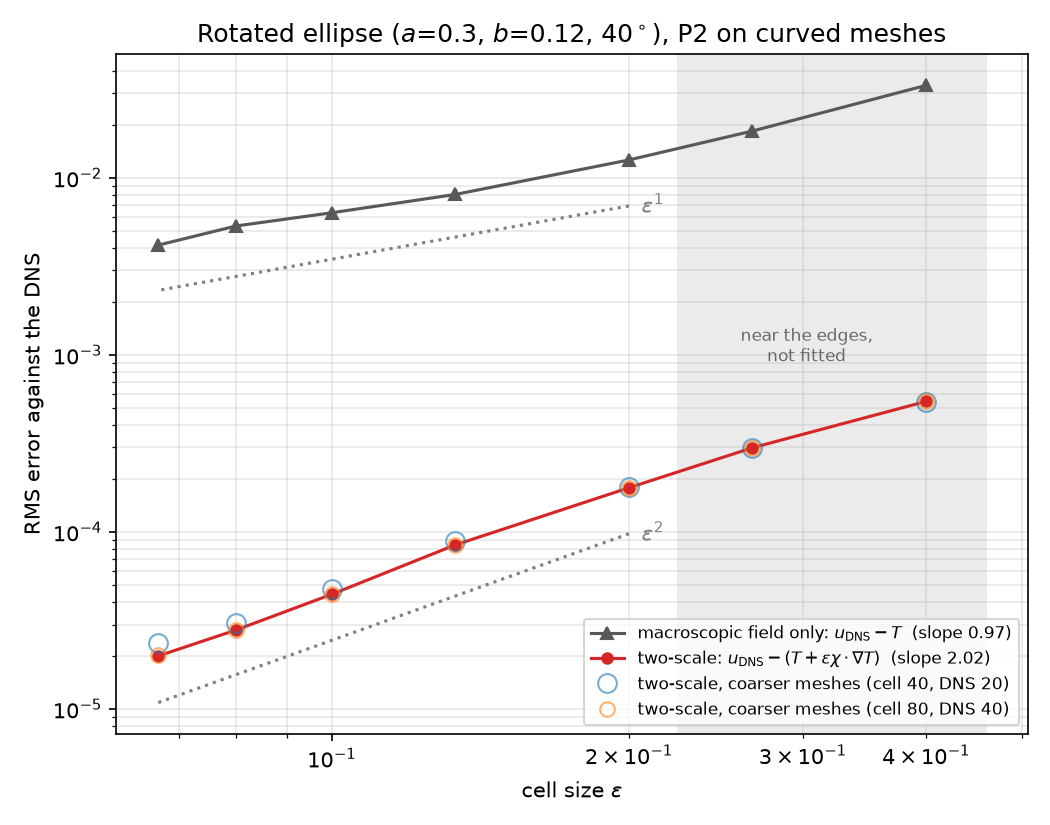
\includegraphics[width=0.7\textwidth]{homogenization_error.png}
  \caption{RMS difference between the DNS and the homogenized fields, as a
  function of the cell size $\varepsilon$, for the rotated ellipse ($a = 0.3$,
  $b = 0.12$, $40^{\circ}$), on a log-log scale. Triangles: macroscopic field $T$
  alone, first order. Filled circles: two-scale reconstruction
  $T + \varepsilon \chi \cdot \nabla T$, second order. Open circles: the same
  reconstruction error computed on the two coarser mesh levels; their
  agreement with the finest level shows that the FEM error is negligible.
  Slopes are fitted over $n \geq 4$; the shaded points ($n = 2, 3$) are
  affected by the boundary layers. Dotted lines: $\varepsilon^1$ and
  $\varepsilon^2$ references. This is the central quantitative result of the
  study. Generated by \texttt{scripts/04\_homogenization\_error.py}.}
  \label{fig:homogenization_error}
\end{figure}

Two checks support this reading. The first concerns the finite element error. The cell
and DNS meshes were refined in three levels, from $1.5/40$ to $1.5/120$ on the unit cell
and from $\varepsilon/20$ to $\varepsilon/60$ in the DNS, and the open circles of
Fig.~\ref{fig:homogenization_error} show that even the coarser levels lie close to the
finest one. Between the last two levels the reconstruction error changes by at most one
percent, so the plotted error is the homogenization error and not a discretization
artefact. The second check concerns the two largest cells, $n = 2$ and $3$, which are
left out of the fit. The sampling region keeps a distance of $0.15 L = 0.12$ from the
edges, which is less than one cell for these sizes, so the sampled points reach into the
boundary layers of Section~\ref{sec:boundary_layer}, and with so few cells the expansion
is in any case far from its asymptotic regime. The figure shows these two points
departing from the second-order trend set by the smaller cells.

\paragraph{Effective conductivity: convergence of the full tensor.} The second
comparison concerns $\kappa^{\star}$ itself. An earlier version of this study compared
$\kappa^{\star}_{11}$ with the effective conductivity read off the DNS of
Eq.~\eqref{eq:bc} for a circular hole, and found a relative difference that did not
decrease with $\varepsilon$. In light of the discussion above this is no surprise, since
for the circle the homogenized solution is exact, and the comparison could only measure
the relative FEM error, which Section~\ref{sec:p2} showed to be constant. For an
anisotropic hole the flux of Eq.~\eqref{eq:bc} is moreover not $\kappa^{\star}_{11}$,
because the insulated top and bottom edges interact with the off-diagonal coupling. We
therefore compare $\kappa^{\star}$ with the apparent tensor of a finite sample defined in
Eq.~\eqref{eq:Kapp}. As shown in Section~\ref{sec:boundary_layer}, the two differ only
through the flux of the boundary layer, by an amount predicted by
Eq.~\eqref{eq:Kapp_rate} to be proportional to $4\varepsilon/L$, with a constant that
does not depend on $n$.

Figure~\ref{fig:tensor_convergence} shows the relative difference
$\|\kappa^{\mathrm{app}} - \kappa^{\star}\|_F / \|\kappa^{\star}\|_F$ for the circle and
the rotated ellipse, with $\kappa^{\star}$ computed on a fine unit-cell mesh. For both
shapes it decreases at the fitted rate $\varepsilon^{1.00}$, with no sign of a plateau.
The prediction of Eq.~\eqref{eq:Kapp_rate} holds in its sharper form as well. Dividing
the relative difference by the area fraction $4\varepsilon/L$ of the layer gives the same
number at every $n$, $4.28\times10^{-3}$ for the circle and $6.3\times10^{-4}$ for the
ellipse, to within one percent. This holds even at $n = 2$, where the corners make up a
large part of the layer but, being of higher order, still do not show.

The right panel of the figure follows the two diagonal entries of the ellipse separately.
They converge at the same rate, and both differences are positive in every case, the
finite sample always conducting slightly better than the effective material. The
off-diagonal entry, which is not plotted, is reproduced about a thousand times more
closely, at the level of the remaining FEM error, so that its rate cannot be resolved.
Each DNS was also run at the two mesh resolutions $\varepsilon/30$ and $\varepsilon/60$,
and given the $h^4$ convergence of these energy quantities, the difference between the
two places the FEM error of the finer level at about one percent of the smallest
difference measured.

\begin{figure}[h]
  \centering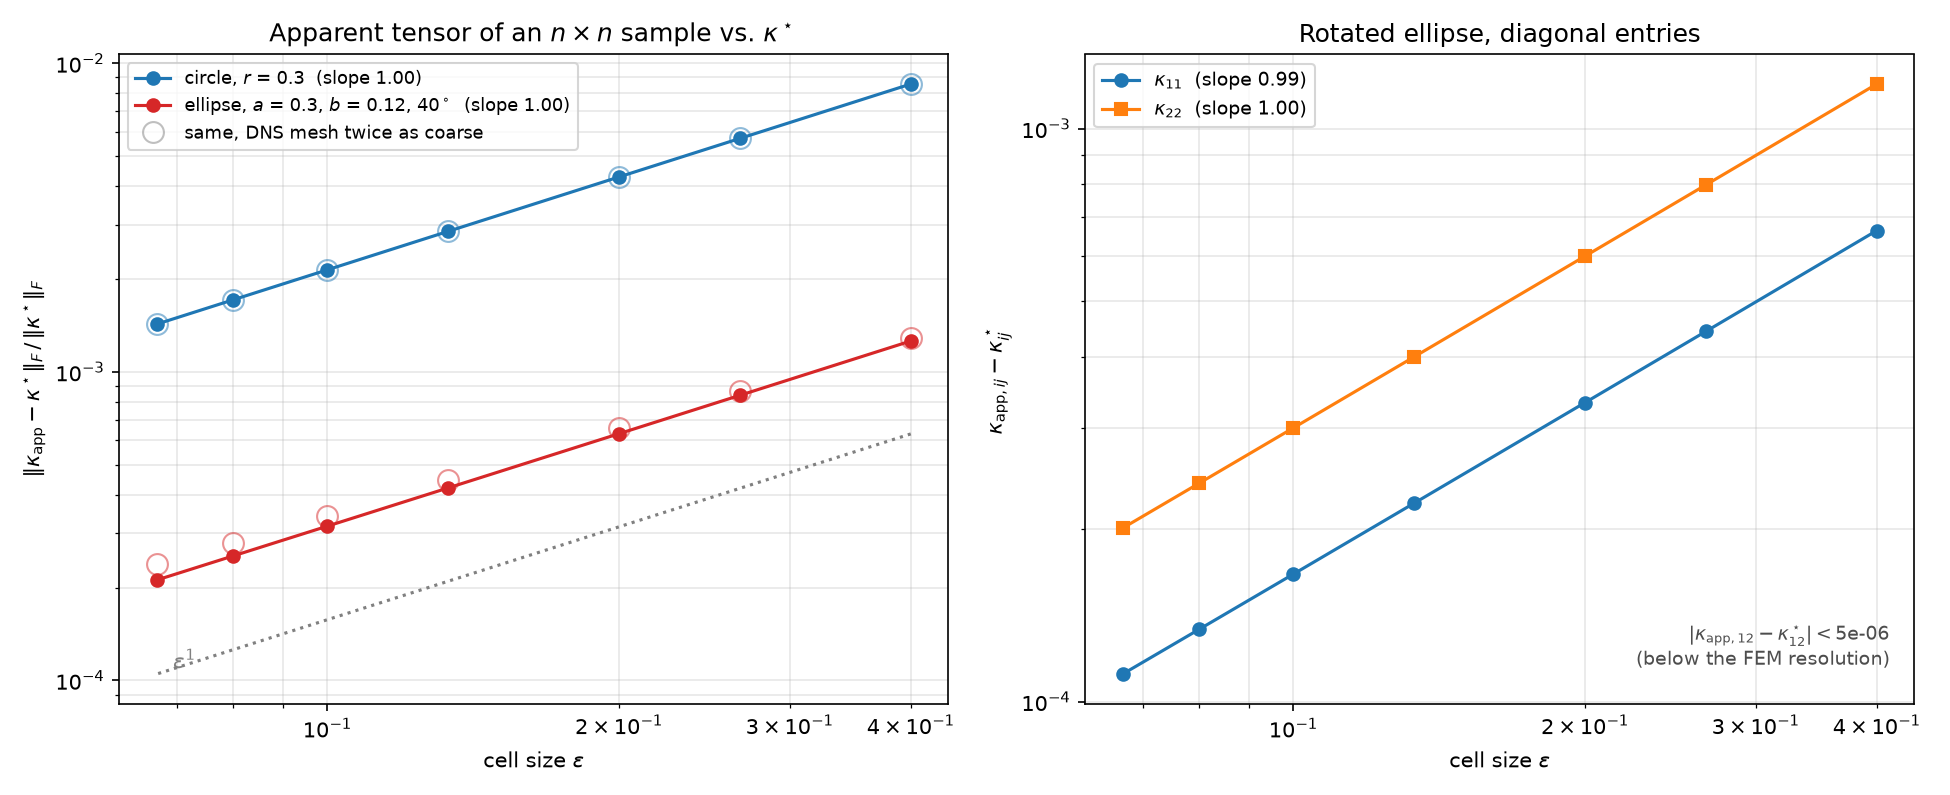
\includegraphics[width=\textwidth]{tensor_convergence.png}
  \caption{Left: relative difference between the apparent tensor
$\kappa^{\mathrm{app}}$ of an $n \times n$ perforated sample (DNS with $u = x_j$ on the
outer boundary, Eq.~\eqref{eq:Kapp}) and the effective tensor $\kappa^{\star}$,
as a function of the cell size, for a circle ($r = 0.3$) and the rotated
ellipse ($a = 0.3$, $b = 0.12$, $40^{\circ}$). Filled symbols: DNS element size
$\varepsilon/60$; open symbols: $\varepsilon/30$. Both decrease as $\varepsilon^1$, the
width of the boundary layer. Right: the diagonal entries for the ellipse,
$\kappa^{\mathrm{app}}_{ii} - \kappa^{\star}_{ii}$, positive in every case; the off-diagonal entry differs by less than $5\times10^{-6}$. Generated by
  \texttt{scripts/05\_tensor\_convergence.py}.}
  \label{fig:tensor_convergence}
\end{figure}

The running times of the two approaches were not measured in this study.
Comparing them on a fixed plate as the number of holes increases would show
directly how much the homogenized pipeline saves, since its cost should not
depend on $\varepsilon$, whereas the cost of the DNS grows quickly with the
number of holes. Such a comparison would be simple to add to the existing
scripts.

\section{Conclusion}

This study implemented a first-order periodic homogenization method for steady-state heat
conduction in a plate perforated by insulating holes, validated it against a direct
numerical solve, and used it to study how the shape of the holes determines the effective
conductivity tensor. The direct solve served both as a benchmark and as a motivation,
since its cost and the complexity of its geometry grow quickly with the number of holes.
The homogenized model replaces it by a single unit-cell problem, from which the effective
tensor $\kappa^{\star}$ is computed, followed by a solve on a plain mesh without holes.

The comparison with a direct solve on an exactly matching tiling confirms the two rates
predicted by the two-scale expansion. For a rotated elliptical hole, the macroscopic field
alone approximates the DNS to first order in $\varepsilon$, and the reconstruction that
adds the corrector term $\varepsilon \chi \cdot \nabla T$ to second order, so that at the
smallest cell size tested it is about two hundred times more accurate. The conductivity
tensor of a finite perforated sample converges to $\kappa^{\star}$ at first order, from
above, for both a circular and an elliptical hole. This rate is set by a boundary layer,
which was measured to decay exponentially over a distance proportional to $\varepsilon$
and therefore occupies a fraction $4\varepsilon/L$ of the sample, a prediction the
measured tensors follow closely. None of this was visible before the discretization was
controlled. With linear elements on meshes tied to $\varepsilon$, the finite element error
does not shrink with $\varepsilon$ and hides both rates behind a plateau, and a circular
hole, for which the homogenized solution happens to be exact with the boundary conditions
used, turned out to test the finite element error rather than the homogenization.

Varying the shape of the hole tunes the effective tensor in a way that follows its
symmetries. At constant porosity, elongating an axis-aligned ellipse raises the
conductivity along its major axis at the expense of its minor axis, and rotating it
produces an off-diagonal entry, which records the sideways deflection of heat by the
tilted hole, vanishes at the axis-aligned orientations and is largest near $45^{\circ}$.

Several extensions follow naturally. Measuring the running times of both approaches would
make the efficiency argument quantitative. The code that tells hole walls apart from
domain edges currently assumes smooth holes such as circles and ellipses, and a small
change would extend it to polygonal holes such as triangles or squares, broadening the
range of shapes that can be studied. The macroscopic domain could also be curved without
difficulty, since the homogenized problem of Eq.~\eqref{eq:macro_problem} places no
requirement on its shape. Finally, the method extends to three dimensions at the cost of a
third corrector and larger meshes, and Figs.~\ref{fig:perforated_cube}
and~\ref{fig:cube_temperature} in the appendix illustrate the geometry such a study would
involve.

\clearpage
\appendix
\section{Additional renderings}

This appendix collects renderings, made with Gmsh and ParaView, that illustrate the
study without being needed for its argument. The three-dimensional ones accompany the
discussion of Section~\ref{sec:domain}, and the plate solutions complement the single-cell
fields of Fig.~\ref{fig:cell_fields}.

\begin{figure}[h]
  \centering
  \begin{minipage}[t]{0.48\textwidth}\centering
    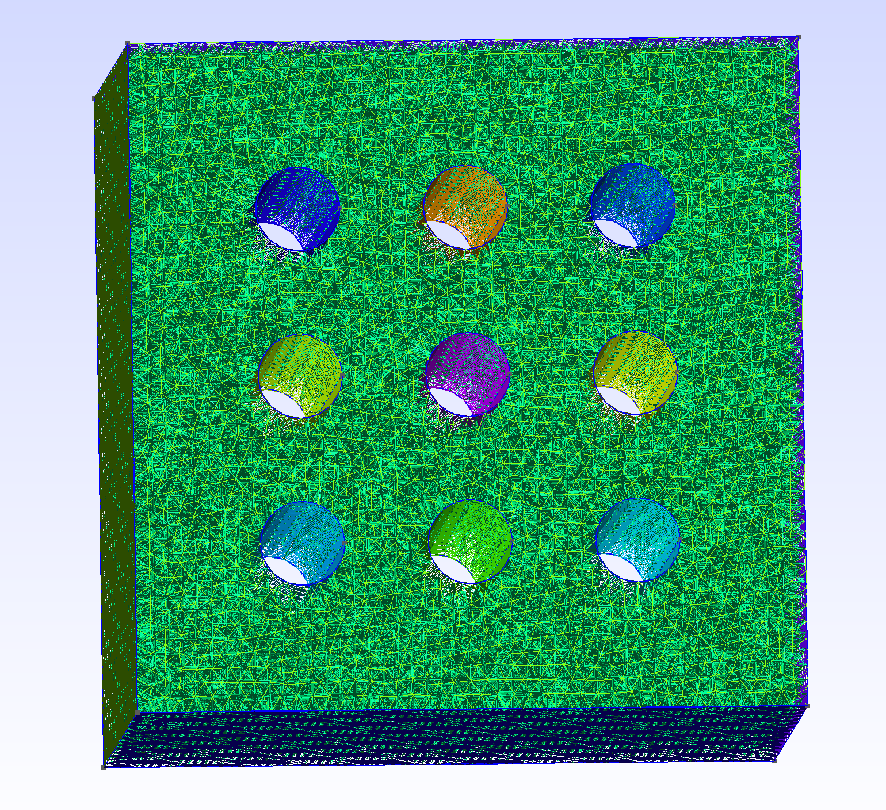
\includegraphics[width=0.85\textwidth]{perforated_cube_mesh.pdf}
    \caption{Mesh of a cube perforated by $3 \times 3$ parallel cylinders,
    opened in Gmsh, with first-order elements.}
    \label{fig:perforated_cube}
  \end{minipage}\hfill
  \begin{minipage}[t]{0.48\textwidth}\centering
    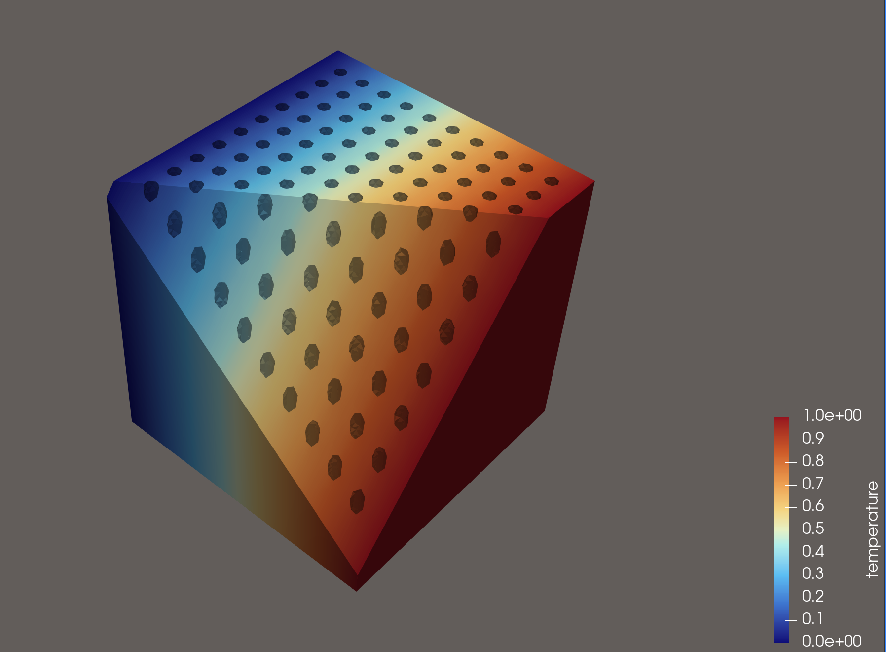
\includegraphics[width=\textwidth]{cube_temperature_slice.pdf}
    \caption{Temperature field on a cube perforated by $10 \times 10$
    parallel cylinders, cut open to show its inside. The temperature varies across the
    cylinders but not along them.}
    \label{fig:cube_temperature}
  \end{minipage}

  \vspace{1.5em}
  \begin{minipage}[t]{0.48\textwidth}\centering
    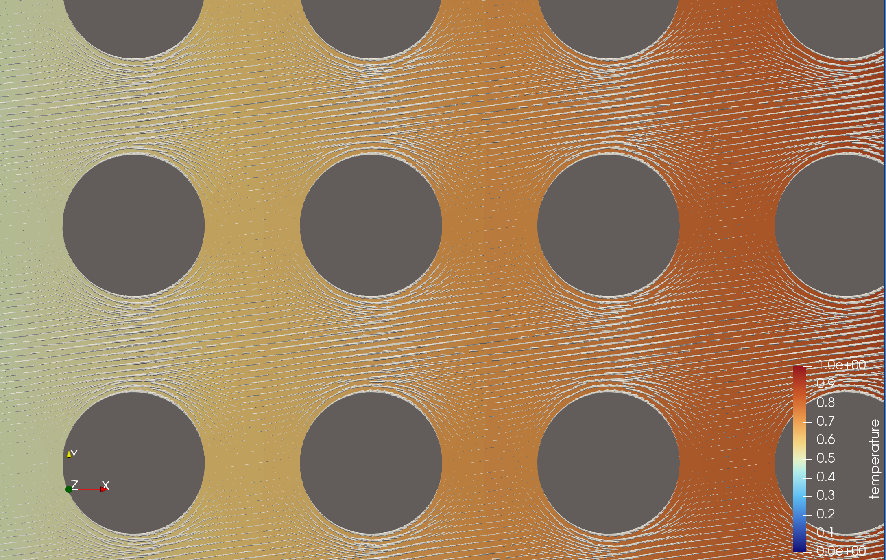
\includegraphics[width=\textwidth]{temperature_circle.pdf}
    \caption{Temperature field and local heat flux, shown by arrows, over a
    whole plate perforated by circular holes. Parameters are $\kappa_{\tmop{solid}} = 1.0$, hole
    radius $0.3$, $10$ holes per side on the domain $L_1 = L_2 = 1.0$, so that
    $\varepsilon = L_1 / 10$, which give $\kappa^{\star} =
    \begin{pmatrix} 0.56 & \approx 0 \\ \approx 0 & 0.56 \end{pmatrix}$, isotropic and
    diagonal as expected for a circular hole.}
    \label{fig:temp_circle}
  \end{minipage}\hfill
  \begin{minipage}[t]{0.48\textwidth}\centering
    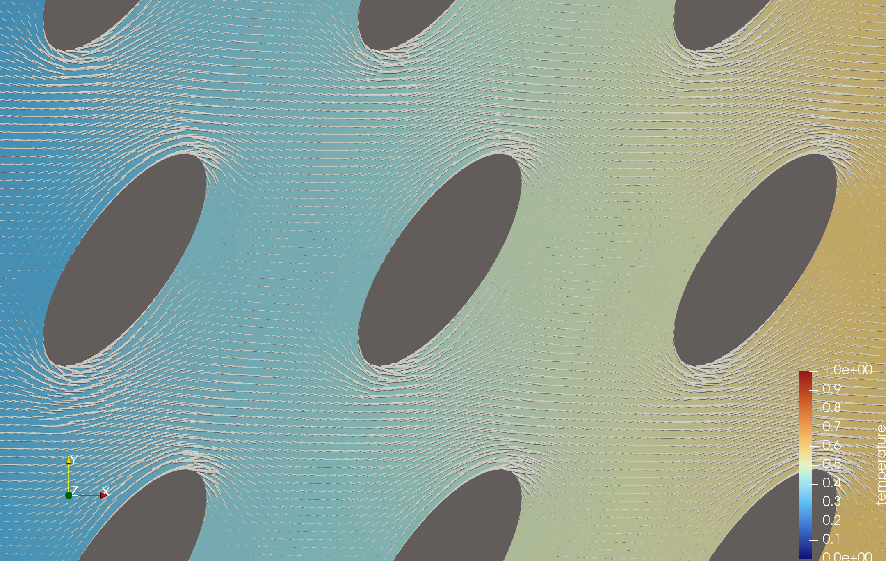
\includegraphics[width=\textwidth]{temperature_ellipse.pdf}
    \caption{Temperature field and local heat flux, shown by arrows, over a
    whole plate perforated by elliptical holes. Parameters are $\kappa_{\tmop{solid}} = 1.0$, ellipse
    semi-axes $a = 0.4$ and $b = 0.15$ rotated by $55^{\circ}$, $10$ holes per side on
    the domain $L_1 = L_2 = 1.0$, so that $\varepsilon = L_1 / 10$, which give
    $\kappa^{\star} = \begin{pmatrix} 0.59 & 0.12 \\ 0.12 & 0.69 \end{pmatrix}$. The
    flux is largest near the tips of the major axis, where the heat is forced to curve
    most sharply around the hole.}
    \label{fig:temp_ellipse}
  \end{minipage}
\end{figure}

\clearpage
\listoffigures

\end{document}
